% Interaction diagram, LaTeX user level and TeX system software level
% Author: Agostino De Marco
% Based on diagram from Marco Miani and Pascal Seppecher.
\documentclass{article}
\usepackage{tikz}
%%%<
\usepackage{verbatim}
\usepackage[active,tightpage]{preview}
\PreviewEnvironment{tikzpicture}
\setlength\PreviewBorder{5pt}%
%%%>
\usetikzlibrary{positioning}

\newcommand{\yslant}{0.5}
\newcommand{\xslant}{-0.6}
\begin{document}
\begin{tikzpicture}[scale=1.1,every node/.style={minimum size=1cm},on grid]

	% Software level
	\begin{scope}[
		yshift=-120,
		every node/.append style={yslant=\yslant,xslant=\xslant},
		yslant=\yslant,xslant=\xslant
	] 
		% The lower frame:
		\draw[black, dashed, thick] (-1.3,1.0) rectangle (8.2,4.5); 
		% Agents:
		\draw[fill=red]  
			(7.5,2) circle (.1)		%DataManager
			(5,2) circle (.1) 		%bib\TeX
			(2,2) circle (.1) 		%(pdf)\LaTex 
			(-0.5,2) circle (.1);	%FrontEnd
		% Flows:
		\draw[-latex,ultra thick,shorten <=5pt,shorten >=5pt] 
			(-0.5,2) to[out=0,in=-180] (2,2); 						% .tex
		\draw[-latex,ultra thick,shorten <=5pt,shorten >=5pt] 
			(2,2) to[out=0, in=-180] (5,2); 						% .aux
		\draw[-latex,ultra thick,shorten <=5pt,shorten >=5pt] 
			(5,2) to[out=90, in=90] (2,2); 							% .bbl
		%\draw[-latex,ultra thick,shorten <=5pt,shorten >=5pt] 
		%	(-0.5,2) to[out=90,in=-180] (2.7,3.0) to[out=0,in=-180] (6.7,3.0) to[out=0,in=135] (7.5,2); % ps2pdfm
		\draw[-latex,ultra thick,shorten <=5pt,shorten >=5pt] 
			(7.5,2) to[out=-180, in=0] (5,2); 						% .bib
		
		% Labels:
		\fill[black]
			(1.0,2) node[above=-3pt, scale=0.9] {\textsf{\bfseries .tex}}
			(3.5,2) node[above=-5pt, scale=0.9] {\textsf{\bfseries .aux}}
			(3.0,3.5) node[xshift=2ex,below=-5pt, scale=0.9] {\textsf{\bfseries .bbl}}
			(-0.5,2) node[below,scale=.9]{\textsf{\bfseries Front End}}
			(2,2) node[below,scale=.9]{\textsf{\bfseries (pdf)\LaTeX}}
			(5,2) node[below,scale=.9]{\textsf{\bfseries bib\TeX}}
			(6.5,2) node[above=-5pt, scale=0.9] {\textsf{\bfseries .bib}}
			(7.0,2) node[below,scale=.9]{\textsf{\bfseries Data Manager}};	
	\end{scope}
	% vertical lines for linking agents on the 2 levels
	\draw[thick](6.3,5.1) to (6.3,0.9);
	\draw[thick](3.8,4) to (3.8,-0.32);
	\draw[thick](0.8,2.4) to (.8,-1.8);
	\draw[thick](-1.70,1.02) to (-1.70,-3);
	
	% User level
	\begin{scope}[
		yshift=0,
		every node/.append style={yslant=\yslant,xslant=\xslant},
		yslant=\yslant,xslant=\xslant
	]
		% The upper frame:
		\fill[white,fill opacity=.70] (-3.1,0) rectangle (9.9,6); % Opacity
		\draw[black, dashed, thick] (-3.1,0) rectangle (9.9,6); 
		 % Agents:
		\draw [fill=red]
			(7.5,2) circle (.1) 	% mendeley
			(5,2) circle (.1) 		% bash
			(2,2) circle (.1) 		% bash
			(-0.5,2) circle (.1);	% Kile

		% the icons
		\node[anchor=south,inner sep=0,xshift=-20pt,yshift=10pt,fill=white] at (-0.5,2)
			{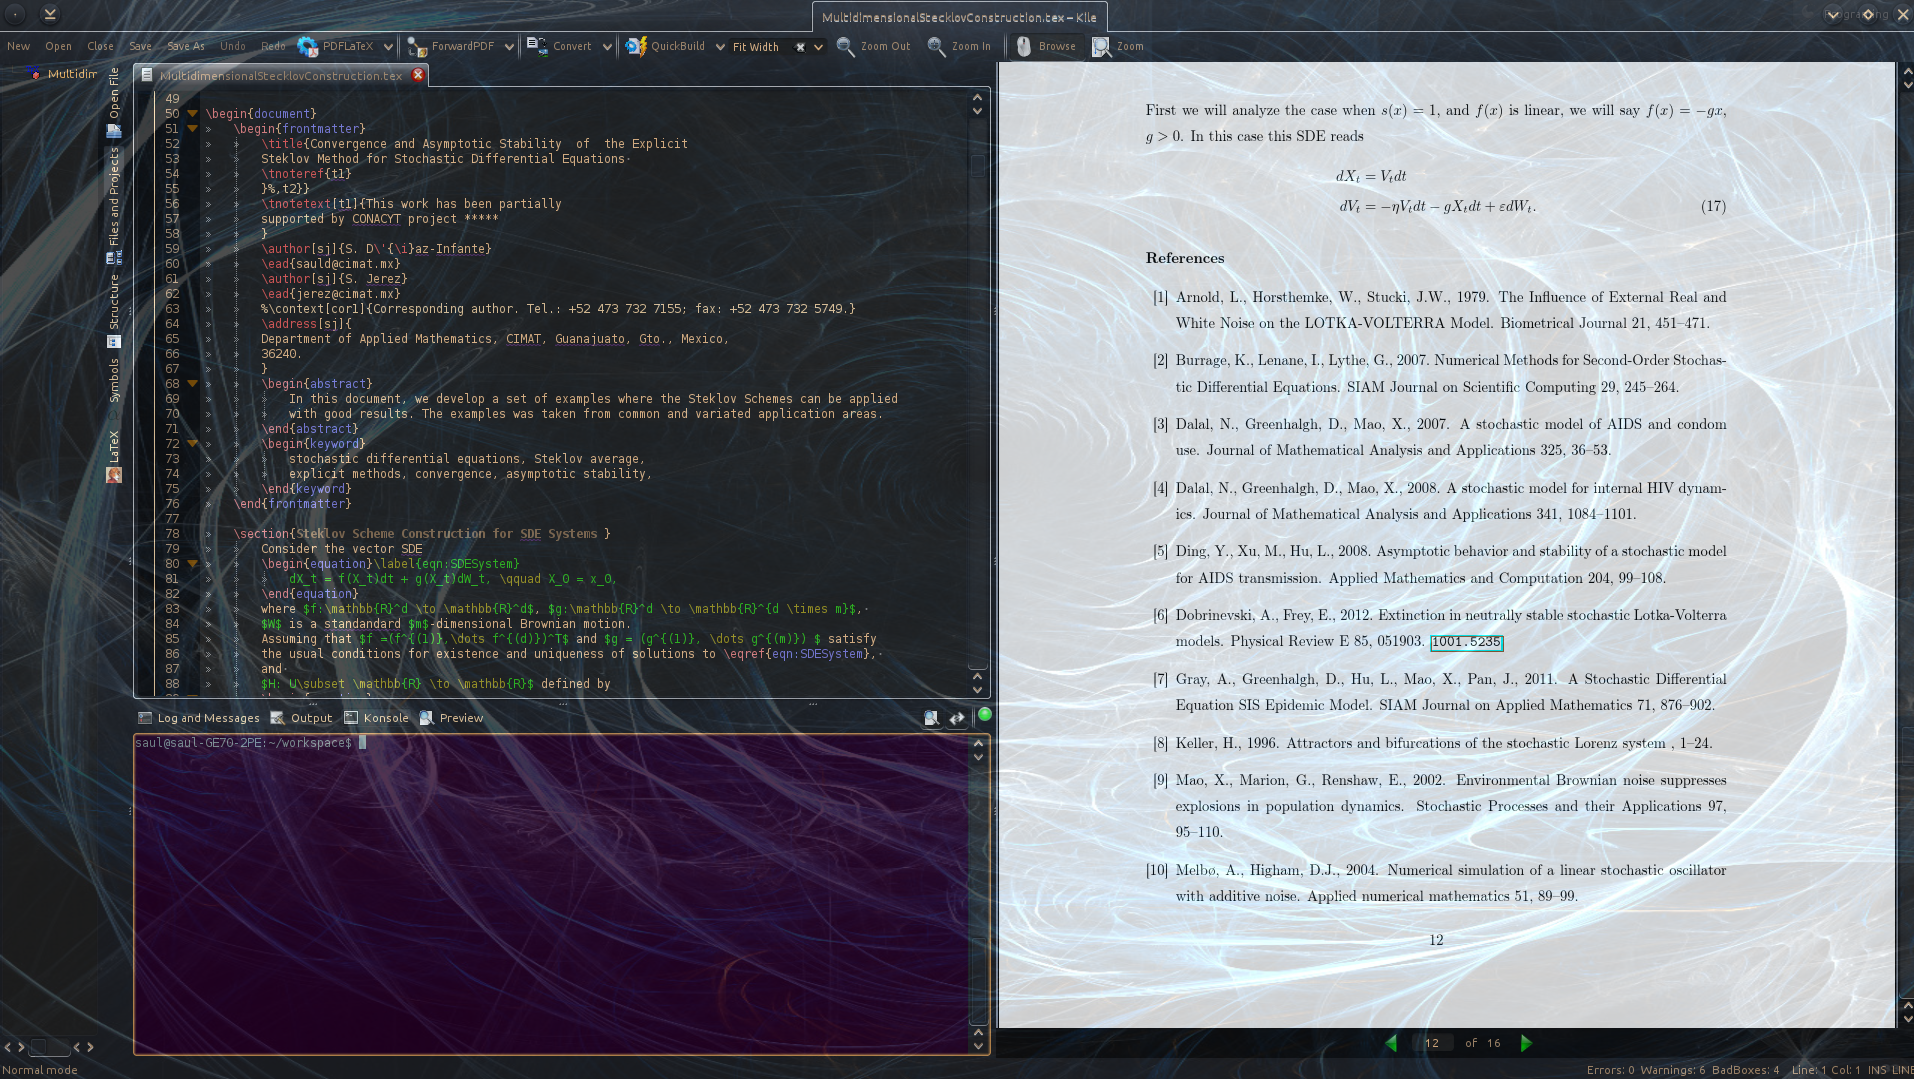
\includegraphics[width=3.0cm]{Kile.png}};
		\node[anchor=south,inner sep=0,xshift=0pt,yshift=8pt] at (2,2)
			{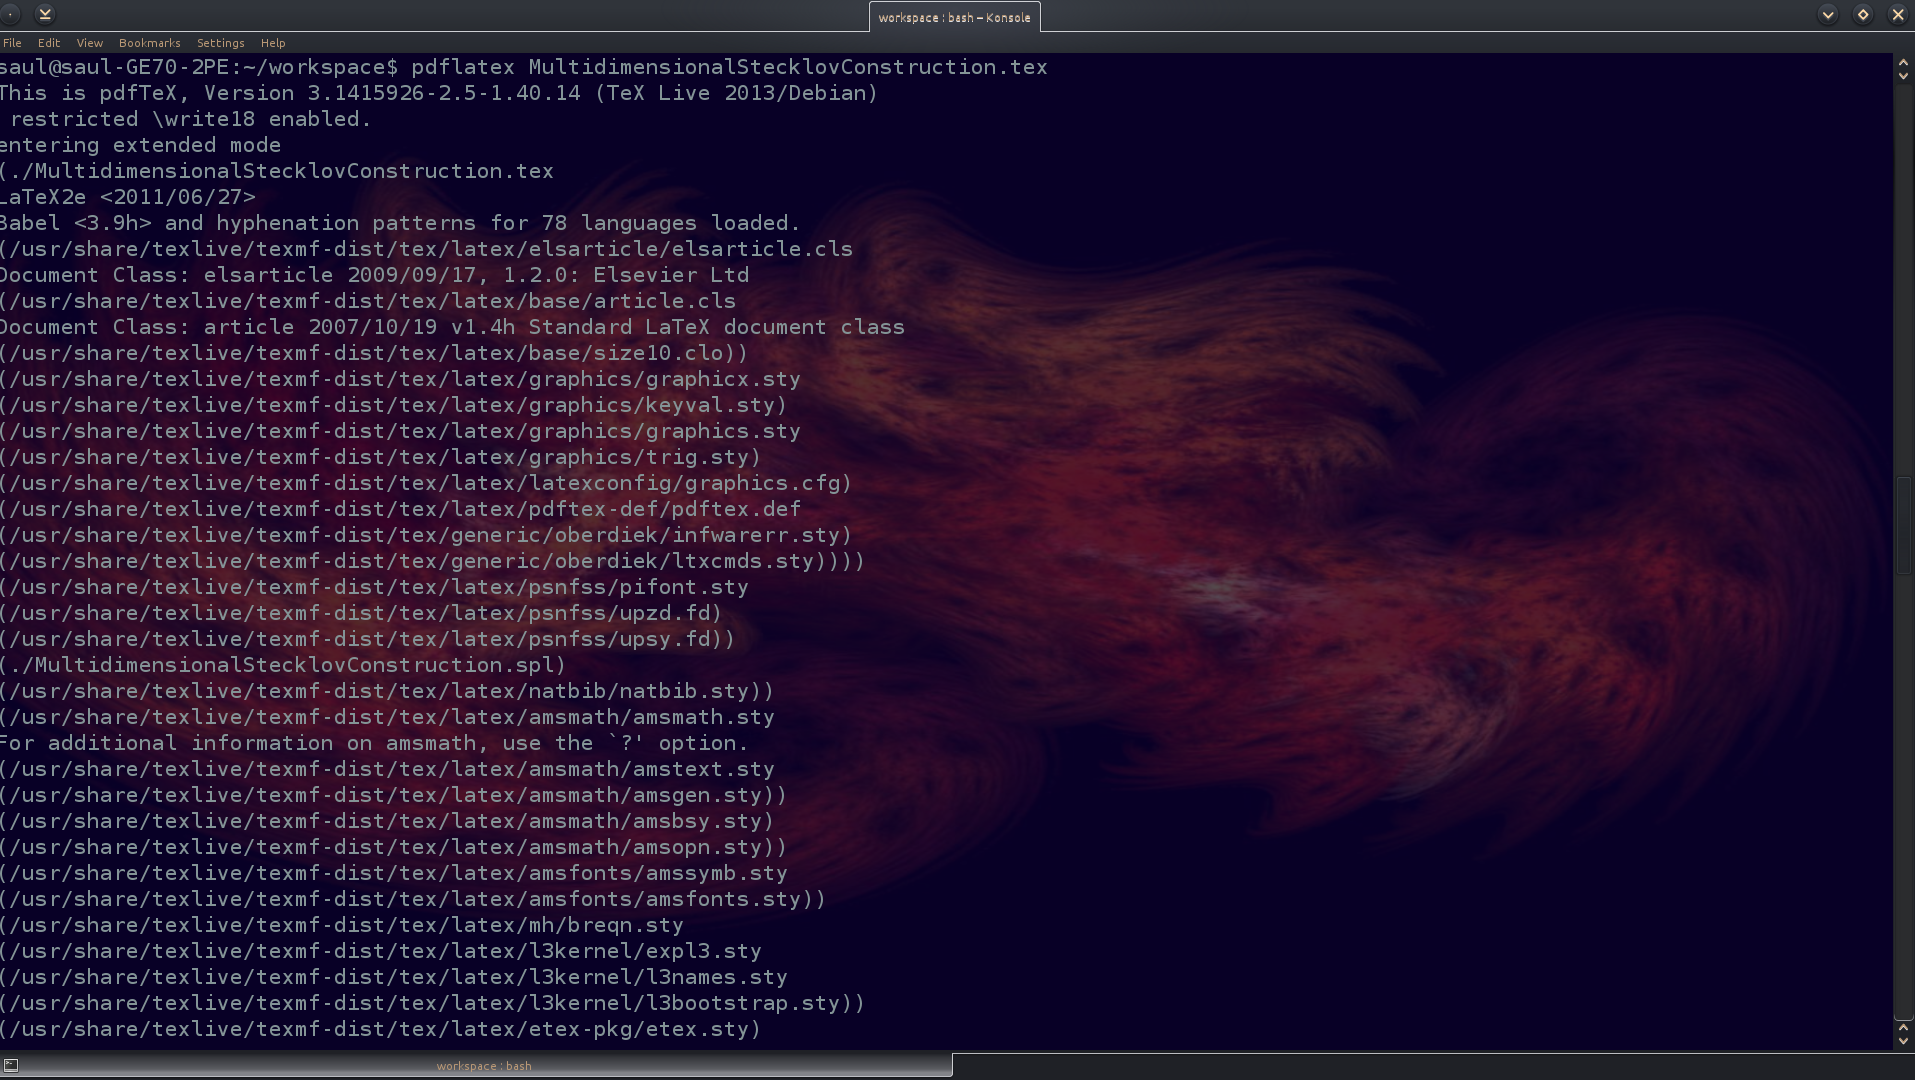
\includegraphics[width=3.0cm]{pdflatexBash.png}};
		\node[anchor=south,inner sep=0,xshift=-5pt,yshift=8pt] at (5,2)
			{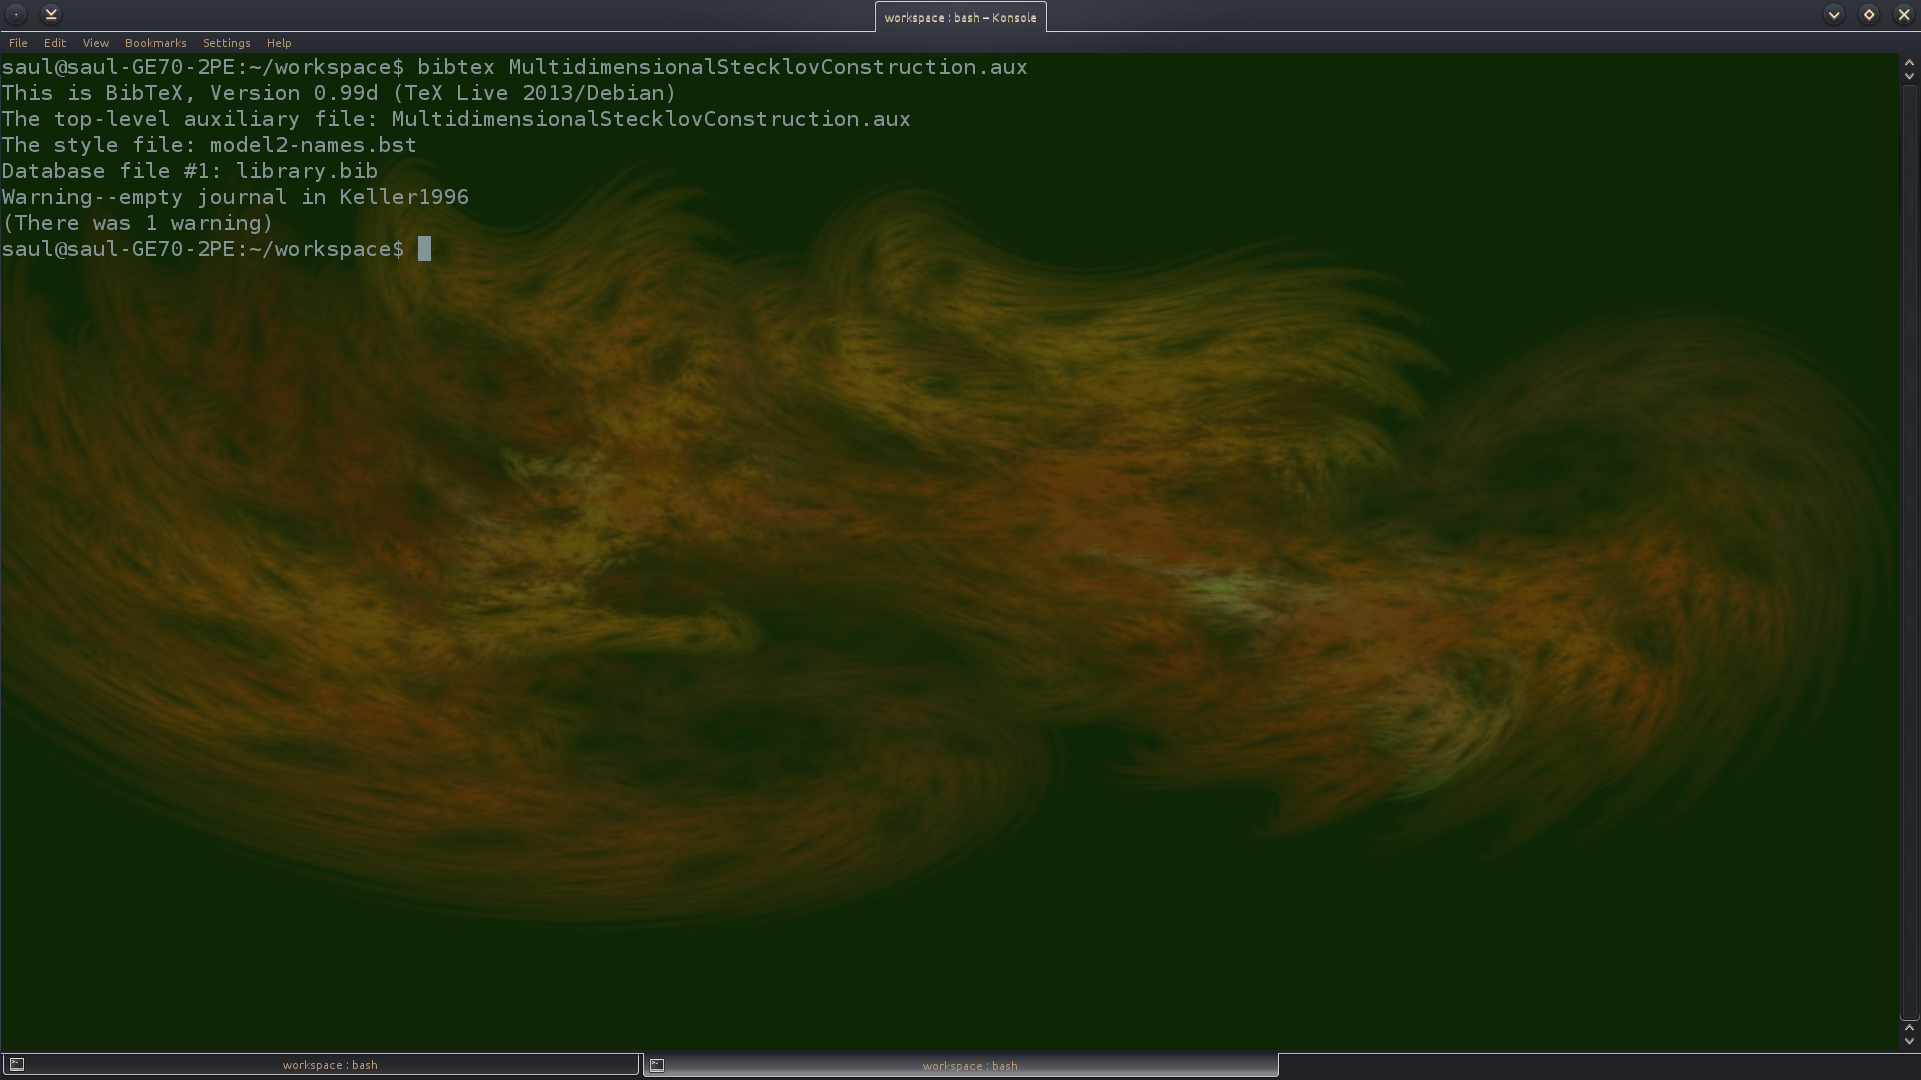
\includegraphics[width=3.0cm]{bibtexBash.png}};
		\node[anchor=south,inner sep=0,xshift=20pt,yshift=8pt] at (7.5,2)
			{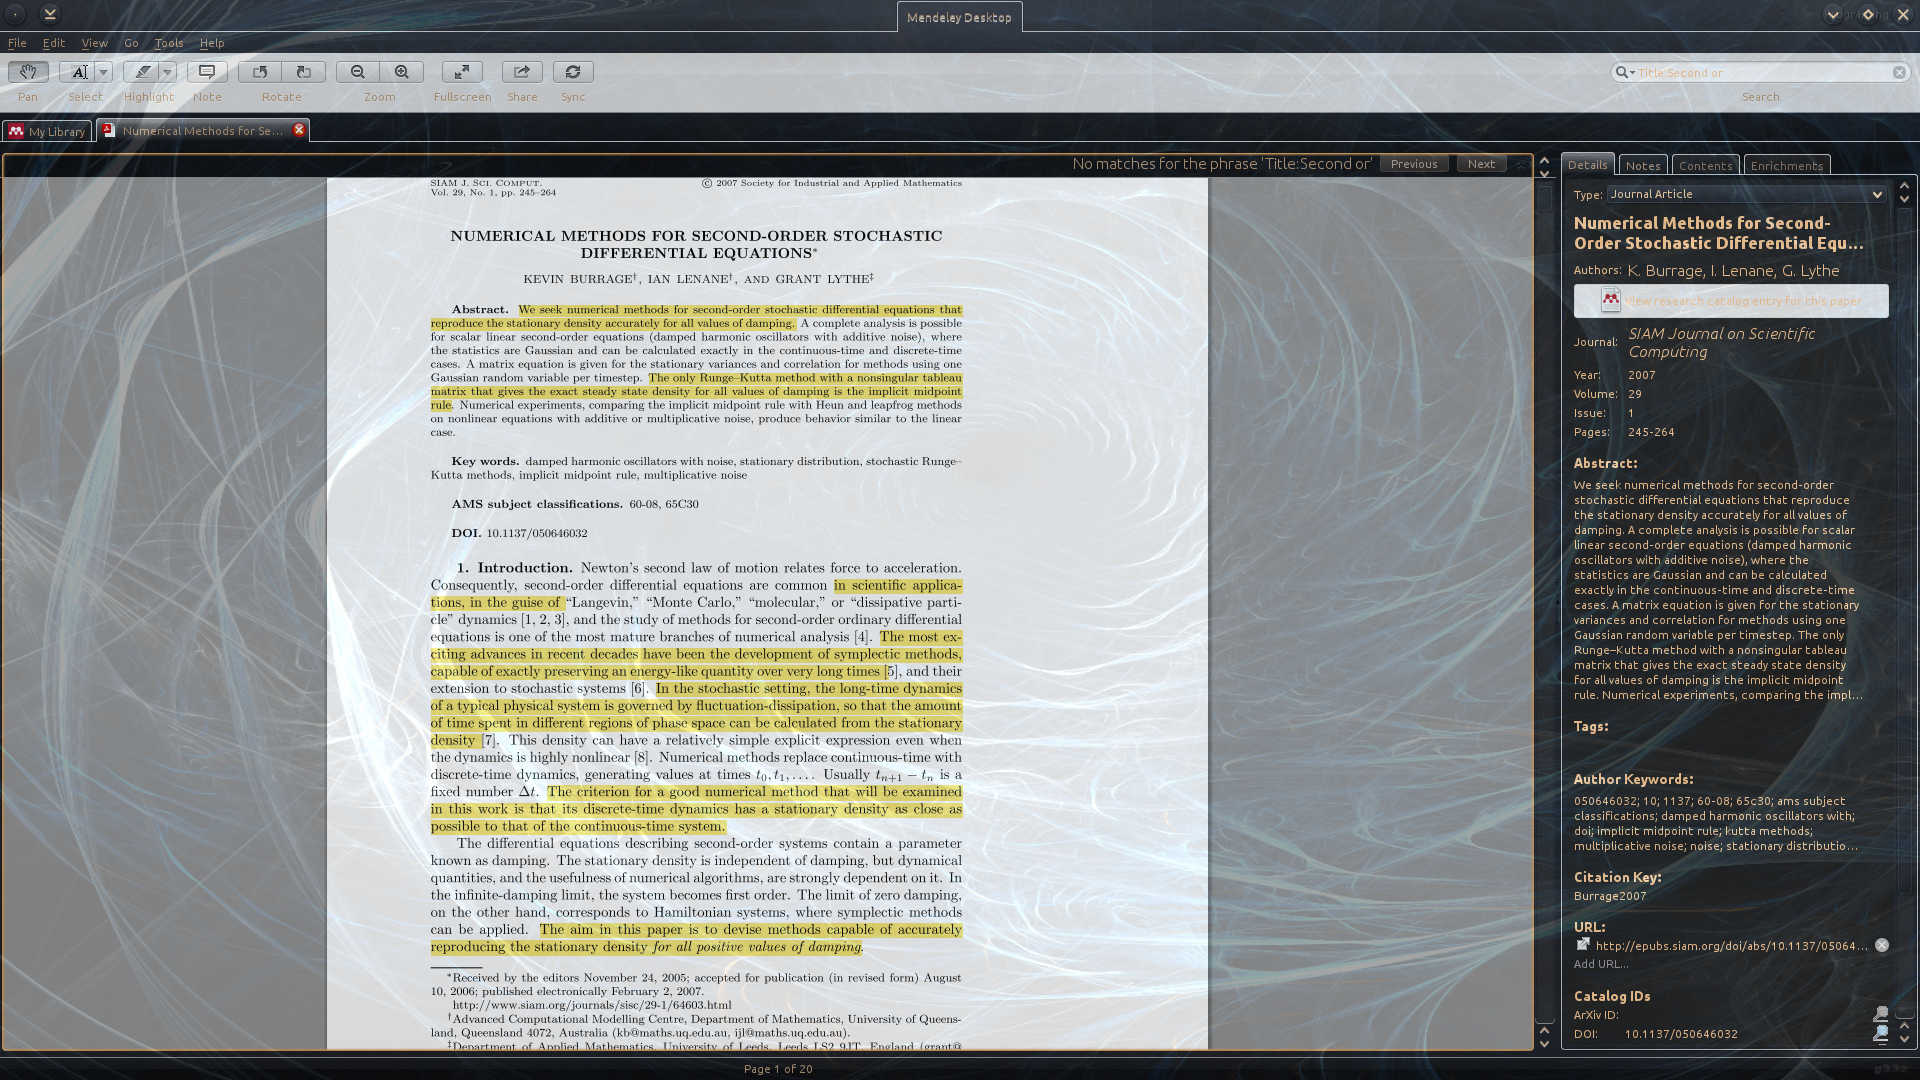
\includegraphics[width=3.0cm]{mendeley.png}};

		\fill[black]
			(7.5,2) node[below right,,xshift=-20pt,yshift=-5pt,scale=.9,text width=2.5cm,align=left,fill=white]
				{\textsf{\bfseries \mbox{Mendeley}}\\ \textsf{\bfseries Calibre}
				\\ \textsf{\bfseries JabRef}}
			(-2.5,5.5) node[anchor=west,inner sep=0, scale=1.1] {\textbf{User level}}
			(5.1,1.9) node[below right,xshift=-20pt,scale=.9,text width=2cm,align=left,fill=white]
				{\textsf{\bfseries bibtex archive.aux}}
			(1.9,1.9) node[below right,xshift=-10pt,scale=.9,text width=2cm,align=left,fill=white]
				{\textsf{\bfseries pdflatex archive.tex}}
			(-0.5,2) node[below right,xshift=-20pt,yshift=-5pt,scale=.9,text width=2.5cm,align=left,fill=white]
				{\textsf{\bfseries \TeX{studio}}\\ \textsf{\bfseries \TeX{maker}}\\
					\textsf{\bfseries \mbox{Kile}}} 
			;
	\end{scope} 
\end{tikzpicture}
\end{document}